\chapter{Corrosion Classification}
\section{Extreme environments}
We study the influence of slow and fast chemistry on structures. Mediated through chemistry that occurs on the surface of materials. This is generally through electrochemical processes that are generally associated with corrosion. Corrosion covers a vast area of material science so we must first go through some of the key electrochemical processes which we cover in this lecture. We are generally interested in the long term view.
\section{Corrosion}
Corrosion is defined as the conversion of metal to a more chemically stable form by chemical and / or electrochemical reaction with their environment. Metals are susceptible because they are good conductors. Corrosion degrades the useful properties of material and structures including strength.
\subsection{Corrosion is similar to a battery}
\begin{figure}[H]
    \centering
    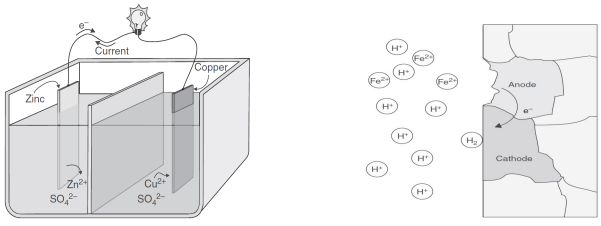
\includegraphics[width = 0.8 \textwidth]{img/figure70.png}
    \caption{Corrosion mechanism compared to battery.}
\end{figure}
This requires an exchange and so only occurs when there are differences. This is classified as either:
\begin{enumerate}
    \item Two different metals in the same liquid
    \item Two different liquids with the same metal
\end{enumerate}
To understand how to stop corrosion, we will have two choices - either coat materials or understand why reaction occurs. First step is to understand the basics of electrochemistry - chemistry is an exchange of electrons. If something is oxidised then something else must be reduced. Reactivity depends what is in the aqueous mixture in contact with the metal.
\subsection{Electrode potentials}
\begin{figure}[H]
    \centering
    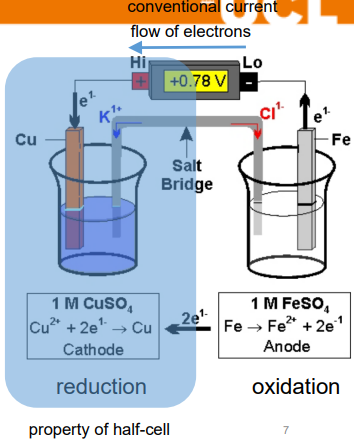
\includegraphics[width = 0.5 \textwidth]{img/figure71.png}
    \caption{Copper reduction and iron oxidation setup in galvanic cell.}
    \label{copperRedIronOx}
\end{figure}
If the iron and copper electrodes are connected electrically, reduction will occur for copper at the expense of the oxidation of iron. \ce{Cu^2+} ions will deposit (electrodeposit) as metallic copper on the copper electrode, while iron dissolves (corrodes) on the other side of the cell and goes into solution.
\begin{align}
    \ce{Fe -> Fe^2+ + 2e^-} \qquad       & \textrm{(oxidation)}        \\
    \ce{Cu^2+ + 2e^- -> Cu} \qquad       & \textrm{(reduction)}        \\
    \ce{Cu^2+ + Fe -> Cu + Fe^2+} \qquad & \textrm{(overall reaction)}
\end{align}
\subsection{Salt bridge}
A salt bridge is used to connect the oxidation and reduction half-cells of a galvanic cell (voltaic cell), a type of electrochemical cell. It maintains electrical neutrality within the internal circuit, preventing the cell from reaction. Salt bridges usually come in two types:
\begin{enumerate}
    \item Glass tube - U-shaped glass tube filled with a relatively inert electrolyte; usually potassium chloride or sodium chloride is used (agar is often used as a gelification agent), although Figure \ref{copperRedIronOx} here illustrates the use of a potassium nitrate solution. The conductivity of the glass tube bridge depends mostly on the concentration of the electrolyte solution. An increase in concentration below saturation increases conductivity. Beyond-saturation electrolyte content and narrow tube diameter may both lower conductivity
    \item Filter paper - the other type of salt bridge consists of filter paper, also soaked with a relatively inert electrolyte, usually potassium chloride or sodium chloride because they are chemically inert. No gelification agent is required as the filter paper provides a solid medium for conduction. Conductivity of this kind of salt bridge depends on a number of factors: the concentration of the electrolyte solution, the texture of the filter paper and the absorbing ability of the filter paper. Generally smoother texture and higher absorbency equates to higher conductivity
\end{enumerate}
\subsection{Electrochemical considerations}
\subsubsection{Oxidation reaction}
Metal atoms characteristically lose or give up electrons in what is called an oxidation reaction.
\begin{equation}
    \ce{M -> M^n+ + ne^-}
\end{equation}
where \ce{n} is valence (number of valent electrons). the site at which oxidation takes place is called the anode. Oxidation is sometimes called an anodic reaction. Example:
\begin{gather}
    \ce{Fe(s) -> Fe^2+(aq) + 2e^-}\\
    \ce{Al(s) -> Al^3+(aq) + 3e^-}
\end{gather}
\subsubsection{Reduction reaction}
The electrons from each oxidised metal atom must be transferred to and become a part of another chemical species in what is termed a reduction reaction. In acid solutions, which have a high concentration of hydrogen ions:
\begin{equation}
    \ce{2H^+ + 2e^- -> H2(g)}
\end{equation}
pH = $- \log_{10}\left[\ce{H^+}\right]$, where more \ce{H^+} results in pH $<$ 7. For an acid solution having dissolved oxygen:
\begin{equation}
    \ce{O2 + 4H^+ + 4e^- -> 2H2O}
\end{equation}
For a neutral or basic aqueous solution in which oxygen is dissolved:
\begin{equation}
    \ce{O2 + 2H2O + 4e^- -> 4OH^-}
\end{equation}
Any metal ions present in the solution may be reduced:
\begin{gather}
    \ce{M^n+ + ne^- -> M}
\end{gather}
The location at which reduction occurs is called the cathode. It is possible for two or more of the reduction reactions to occur simultaneously.
\subsection{Galvanic couple}
Two metals electrically connected in a liquid electrolyte wherein one metal becomes an anode and corrodes while the other acts as a cathode.

The question is which one corrodes. An electric potential or voltage will exist between the two cell halves, and its magnitude can be determined if a voltmeter is connected in the external circuit. Various electrode pairs have different voltages; the magnitude of such a voltage may be thought of as representing the driving force for the electrochemical oxidation-reduction reaction.
\begin{align}
    \ce{Cu^2+ + Fe -> Cu + Fe^2+} \quad & \left(\SI{0.780}{\volt}\right) \\
    \ce{Fe^2+ + Zn -> Fe + Zn^2+} \quad & \left(\SI{0.323}{\volt}\right)
\end{align}
Standard half cell: a half-cell of a metal electrode immersed in a \ce{1M} solution of ions and at \SI{25}{\degree C}. To understand reaction, we have to look at one half of the electrochemical cell or half-battery, specifically when one half of the battery is a standard form.
\section{Standard hydrogen reference probe}
It consists of an inert platinum electrode in a \ce{1M} solution of \ce{H^+} ions, saturated with hydrogen gas that is bubble through the solution at a pressure of \SI{1}{atm} and a temperature of \SI{25}{\degree C}.

\textbf{Standard electromotive force (emf) series.} It is generated by coupling to the standard hydrogen electrode, standard half-cells for various metals and ranking them according to the measured voltage. This tells us the potential for reaction but not the rate.
\begin{figure}[H]
    \centering
    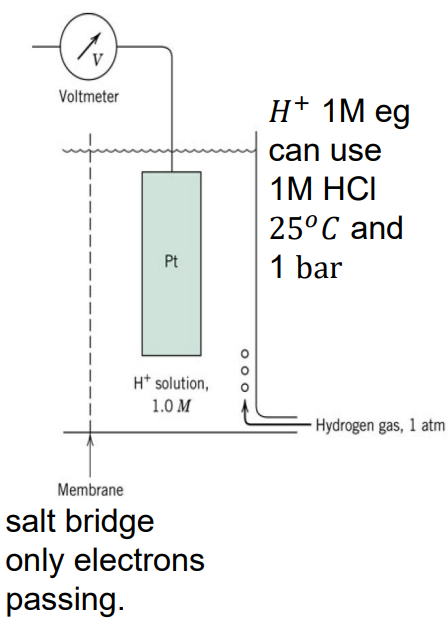
\includegraphics[width = 0.5 \textwidth]{img/figure72.png}
    \caption{Standard hydrogen reference probe.}
\end{figure}